\documentclass[a4paper,titlepage,12pt]{article}

%% Language and font encodings
\usepackage[swedish]{babel}
\usepackage[utf8]{inputenc}
\usepackage{textcomp}
\usepackage{amsmath}
\usepackage{graphicx}
\usepackage[colorinlistoftodos]{todonotes}
\usepackage{afterpage}
\usepackage[colorlinks=true, urlcolor=blue, linkcolor=black, pdfborder={0 0 0}]{hyperref}
\usepackage{longtable}
\usepackage[yyyymmdd]{datetime}
\usepackage[bottom]{footmisc}
\usepackage{titling}
\usepackage{pbox}
\usepackage{booktabs}
\usepackage{color, colortbl}
\definecolor{Gray}{gray}{0.9}
\usepackage{changepage, titlesec}

%Set page size
\usepackage{geometry}
\geometry{margin=3cm}
\usepackage{parskip} 
\setcounter{secnumdepth}{5}

\usepackage{float}


\renewcommand{\dateseparator}{-}
\addto\captionsswedish{% Replace "swedish" with the language you use (if using babel)
  \renewcommand{\contentsname}%
    {Innehållsförteckning}%
}

%%%%%%%%%%%%%%%%%%%%%%%%%%%%%%%
% Header and footer
%%%%%%%%%%%%%%%%%%%%%%%%%%%%%%%

\usepackage{fancyhdr}
\pagestyle{fancy}

\lhead{
\includegraphics[scale=0.3]{images/logga.png}}
\chead{System för 3D-kopiering}
\rhead{\today}
\setlength\headheight{26pt} 


\lfoot{TDDD96 --- PUM}
\rfoot{Grupp 9}

\posttitle{\end{center}}

\begin{document}
\begin{titlepage}

% Title text
\topskip0pt
\vspace*{\fill}
\huge
\textbf{Användarmanual} \\
\Large
System för 3D-kopiering \\
\noindent\rule{17cm}{0.4pt}
\bigskip

\Large
Version: 1.0 \\
\today

\date{\today}
\vspace*{\fill}

% Image 
\vspace*{\fill}
\begin{minipage}[b]{0.7\textwidth}
	
\includegraphics[width=8cm]{images/liu-logga.png}
\end{minipage}
\begin{minipage}[b]{0.4\textwidth}
	\normalsize
	\textit{Linköpings universitet} \\
	\textit{SE-581 83 Linköping, Sverige}\\
	\textit{013-28 10 00, www.liu.se}
\end{minipage}

\end{titlepage}
\newpage
\begin{center}
\pagenumbering{gobble}

\tableofcontents
\newpage

\end{center}

%%%%%%%%%%%%%%%%%%%%%%%%%%%%%%%%%%%%%%%%%%%%%%%%%%%%%%%%%%%%%%%%%%%%%
%					Introduction
%%%%%%%%%%%%%%%%%%%%%%%%%%%%%%%%%%%%%%%%%%%%%%%%%%%%%%%%%%%%%%%%%%%%
\pagenumbering{arabic}
\section{Inledning}
	Detta dokument är en användarmanual för 3D-kopieringsprojektet på Linköpings universitet. Projektet pågick under vårterminen 2017 och utfördes av sju stycken studenter ifrån universitetet. Projektet är en del i kursen TDDD96 - Kandidatprojekt i programvaruutveckling som ges vid Linköpings universitet. Användarmanualen beskriver hur produkten används.
	
	\subsection{Utvecklare}
		Önskas kontakt med någon av utvecklarna så kan följande kontaktuppgifter användas:
		
		\scalebox{0.8}{
			\begin{tabular}{|l|l|l|}
				\hline
				\rowcolor{Gray}
				\textbf{Namn} & \textbf{Ansvar} & \textbf{E-post} \\
				\hline
				Hampus Dunström & Utvecklingsledare & hamdu013@student.liu.se\\
				\hline
				Olof Holmberg & Testledare & oloho254@student.liu.se\\
				\hline
				Gustav Jannering & Analysansvarig & gusja113@student.liu.se\\
				\hline
				Michael Karlsson & Teamledare & micka199@student.liu.se\\
				\hline
				Martin Lundberg & Arkitekt & marlu819@student.liu.se\\
				\hline
				Hannes Tuhkala & Dokumentansvarig \& konfigurationsansvarig & hantu447@student.liu.se\\
				\hline
				Fredrik Wallström & Kvalitetssamordnare & frewa814@student.liu.se\\
				\hline
		\end{tabular}}
		
	\subsection{Definitioner}
		Nedan följer definitioner och ordval som används i denna användarmanual.
		
		\begin{itemize}
			\item ISY - Institutionen för systemteknik
			\item ICP - Iterative closest point (iterativ närmast punkt)
			\item PCL - Point cloud library
		\end{itemize}
    
\newpage  

%%%%%%%%%%%%%%%%%%%%%%%%%%%%%%%%%%%%%%%%%%%%%%%%%%%%%%%%%%%%%%%%%%%%%
%					Använda systemet
%%%%%%%%%%%%%%%%%%%%%%%%%%%%%%%%%%%%%%%%%%%%%%%%%%%%%%%%%%%%%%%%%%%%
\section{Att använda systemet}
	Som användare av systemet finns det två stycken sätt att använda systemet, ett kommandoradsgränssnitt, 3DCopy, samt ett grafiskt användargränssnitt. Med hjälp av dessa gränssnitt är det möjligt att ta en uppsättning av icke kompletta punktmoln för att generera en utskriftsbar 3D-mesh. Gränssnitten är anpassade för att ta in en uppsättning av punktmoln (.pcd-filer). För att använda systemet kan det vara vettigt att filtrera de punktmoln som är tänkta att använda. Därför har det skapas ett filtreringsprogram som filtrerar bort skräppunkter ur ett punktmoln.
	
	\subsection{Att använda TreeD-Wrapper}
	TreeD-Wrapper är ett hjälpprogram som är till för att ta ett flertal skanningar med hjälp av programmet TreeD. Med TreeD-Wrapper kan man ta skanningar från ett antal rotationer på rotationsbordet automatiskt och samtidigt filtrera och placera dessa rätt. TreeD-Wrapper används via ett kommandoradsgränssnitt och kommer spara alla de filtrerade skanningarna i den mappen som användaren står i när den kör programmet. Programmet används som följande:
	
	\texttt{treed\_wrapper.py [options]}
	
	där options består av valfria flaggor att skicka in för att bestämma hur skanningarna och filtreringen ska utföras. Tabell \ref{tab:treedwrapper_flaggor} visar de flaggor som kan skickas in till programmet.
	
	Följande exempel tar 36 skanningar per varv vid 0 och 20 grader på curve (det vill säga 72 skanningar totalt) och visar sedan resultatet i pcl\_viewer:
	
	\texttt{treed\_wrapper.py --view -r 36 -c 0 20}
	
	TreeD-Wrapper är uppbyggd på så sätt att när en skanning misslyckas på grund av att något går fel så kraschar TreeD-Wrapper och säger vad som gått fel. Oftast kan fel lösas genom att starta om hårdvaran och/eller datorn som programmet körs på. TreeD-Wrapper kan sedan köras igen med samma parametrar som innan och kommer då fortsätta från den punkten då programmet kraschade vilket gör att det är enkelt att ta många skanningar även om det underliggande systemet inte alltid är stabilt.
		
	\begin{table}[H]
		\centering
		\caption{Flaggor för TreeD-Wrapper.}
		\label{tab:treedwrapper_flaggor}
		
		\begin{tabular}{p{0.2\linewidth}p{0.6\linewidth}}
			Flagga & Förklaring \\
			\hline
			-h, \texttt{--}help & Skriver ut en hjälptext för TreeD-Wrapper i terminalen. \\
			\hline
			-r, \texttt{--rotation} & Anger hur många skanningar som ska tas på ett varv runt y-axeln. Till exempel ger 36 skanningar per varv att skanningar tas med 10 grader mellan varje. \\
			\hline
			-c, \texttt{--curve} & Anger de rotationer i grader som ska användas för TreeD's curve, det vill säga rotationen kring x-axeln. Skickas in som en lista med rotationer, till exempel kan \texttt{-c 0 10 20} användas för att ta skanningar vid 0, 10 och 20 grader. \\
			\hline
			-w, \texttt{--view} & Öppna de filtrerade punktmolnen i pcl\_viewer då alla skanningar är klara. \\
			\hline
			\texttt{--cutoff\_height} & Anger den \texttt{cutoff\_height} som ska användas vid filtreringen, se avsnitt \ref{sec:filtrering}. \\
			\hline
			-f, \texttt{--filter\_only} & Ta inga nya skanningar utan filtrera endast de skanningar som redan tagits. \\
			\hline
		\end{tabular}
		
	\end{table}
	
	\subsection{Att använda filtreringen}
	\label{sec:filtrering}
	För att använda filtret finns ett separat program som körs genom att anropa \texttt{filter} i terminalen. Användningen av filtret ser ut som följande:
	
	\texttt{filter [options] sources}
	
	där options är valfria flaggor att skicka in till filtret och sources är en eller fler pcd-filer eller mappar med pcd-filer som ska filtreras.
	
	Filtret går igenom alla pcd-filer och mappar som skickas in och filtrerar dem. Då filer skickas in till filtret sparas resultatet i en ny fil med namnet originalnamn\_filtered.pcd och då mappar skickas in skapas en ny mapp med namnet originalnamn\_filtered där de filtrerade filerna sparas.
	
	De flaggor som kan skickas in till programmet visas i tabell \ref{tab:filter_flaggor}.
	
	\begin{table}[H]
		\centering
		\caption{Flaggor för filtret.}
		\label{tab:filter_flaggor}
		
		\begin{tabular}{p{0.2\linewidth}p{0.6\linewidth}}
			Flagga & Förklaring \\
			\hline
			-h, \texttt{--help} & Skriver ut en hjälptext för filtret i terminalen. \\
			\hline
			-r, \texttt{--rotation} & Anger hur mycket det filtrerade punktmolnet ska roteras kring y-axeln i grader. \\
			\hline
			-c, \texttt{--curve} & Anger hur mycket det filtrerade punktmolnet ska roteras kring x-axeln i grader. \\
			\hline
			\texttt{--cutoff\_height} & Anger hur högt upp objektet som skannades satt. Ange ett högre värde för objekt som satt längre ner, d.v.s. närmare bottenplattan på rotationsbordet. \\
			\hline
			-s, \texttt{--scale} & Anger hur mycket objektet ska skalas på bredden för att få rätt proportioner. Det rekommenderas att köra skanningar med cart\_speed=200 och låta denna inställning ha sitt standardvärde (0.5). \\
			\hline
		\end{tabular}
	
	\end{table}

	Filtret kan även användas i vidareutveckling av systemet genom att inkludera klassen \texttt{Filter.h} och använda filtret i C++.
	
	\subsection{Att använda webbapplikationen}
	
	När man ansluter till webbapplikationen kommer man att mötas av ett gränssnitt som liknar det i figur \ref{fig:web_gui}. Det som kan variera är längden av listan med de jobb som är köade, körs eller som är klara.
	
	\begin{figure}[H]
		\centering
		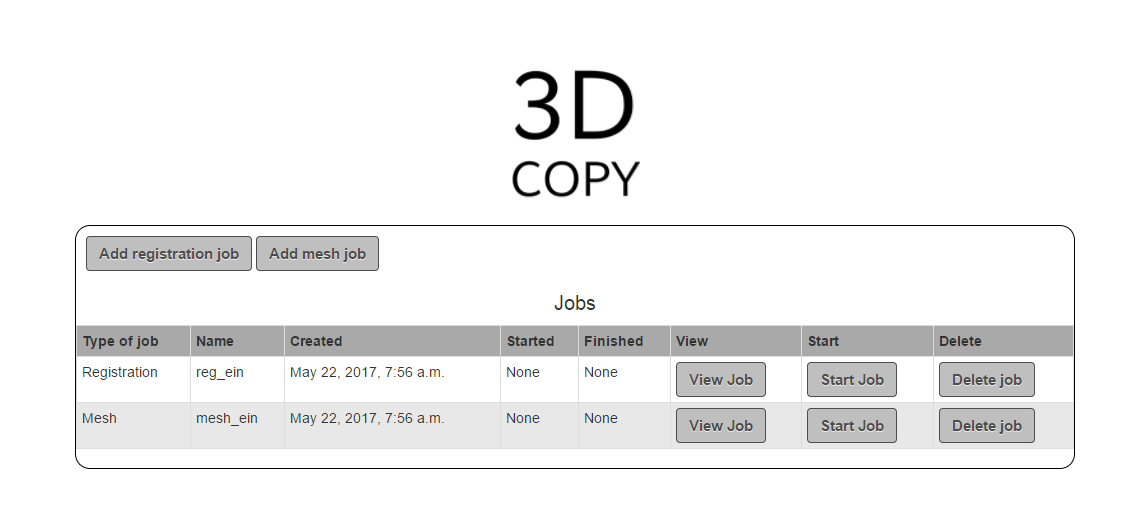
\includegraphics[width=160mm]{images/gui_web.PNG}
		\caption{Webbapplikationens användargränssnitt.}
		\label{fig:web_gui}
	\end{figure}

	Uppe i vänstra hörnet finns knapparna \textit{Add registration job} och \textit{Add mesh job}.
	
	\subsubsection{Add registration job}
	
	Genom att trycka på \textit{Add registration job} så öppnas formuläret för att starta ett registreringsjobb. Formuläret visas i figur \ref{fig:reg_job_form}.
	
	\begin{figure}[H]
		\centering
		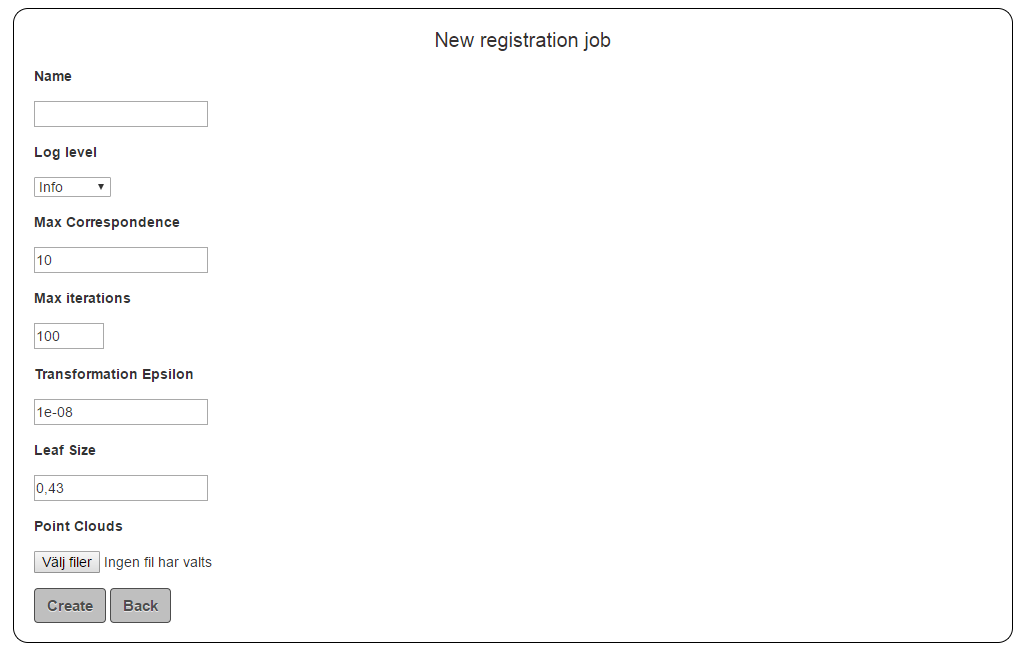
\includegraphics[width=160mm]{images/reg_job_form.PNG}
		\caption{Formuläret för att skapa ett registreringsjobb.}
		\label{fig:reg_job_form}
	\end{figure}

	I formuläret för registreringsjobbet får man först välja namn på jobbet. Därefter får man välja vilken nivå som loggningen ska använda. Sedan ska man välja parametrarna för registreringen. Slutligen så trycker man på \textit{Välj filer} och väljer de filer som ska registreras. Därefter trycker man på \textit{Create} och jobbet kommer då att skapas och skickas till servern och visas i listan i standardvyn. Om man trycker på \textit{Back} så avbryts processen för att skapa ett jobb och man kommer tillbaka till standardvyn som visar listan med jobb.
	
	\subsubsection{Add mesh job}
	
	Om man trycker på \textit{Add mesh job} så öppnas formuläret för att skapa ett meshningsjobb. Formuläret visas i figur \ref{fig:mesh_job_form}.
	
	\begin{figure}[H]
		\centering
		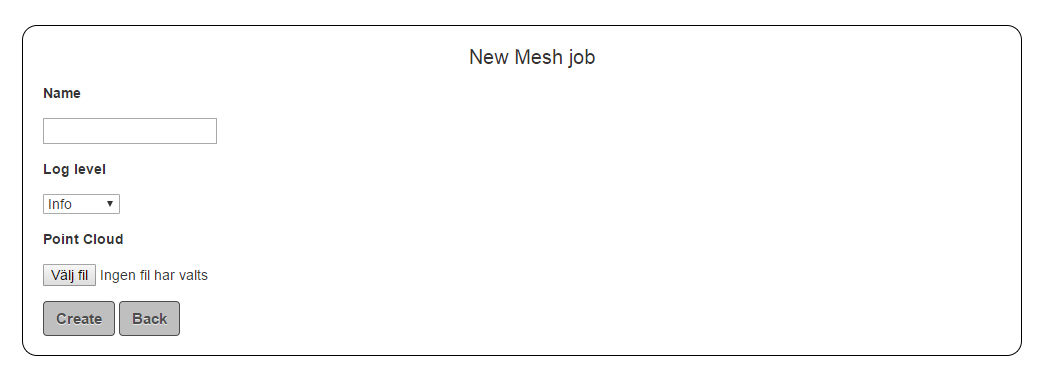
\includegraphics[width=160mm]{images/mesh_job_form.PNG}
		\caption{Formuläret för att skapa ett meshningsjobb.}
		\label{fig:mesh_job_form}
	\end{figure}

	I formuläret för meshningsjobbet får man först välja namn på jobbet. Därefter får man välja vilken nivå som loggningen ska använda. Slutligen så får man välja vilken fil som ska meshas. Därefter trycker man på \textit{Create} och jobbet kommer då att skapas och skickas till servern och visas i listan i standardvyn. Om man trycker på \textit{Back} så avbryts processen för att skapa ett jobb och man kommer tillbaka till standardvyn som visar listan med jobb.
	
	\subsubsection{Jobblistan}
	
	När ett jobb är skapat så kommer det att visas i listan över existerande jobb. Hur ett jobb i listan ser ut visas i figur \ref{fig:job_in_list}.
	
	\begin{figure}[H]
		\centering
		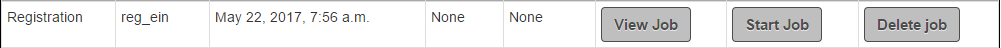
\includegraphics[width=160mm]{images/job_in_list.PNG}
		\caption{Ett jobb i jobblistan.}
		\label{fig:job_in_list}
	\end{figure}

	I första kolumnen visas vilken typ av jobb det är, i detta fall är det ett registreringsjobb. I andra kolumnen visas när jobbet skapades. I tredje kolumnen visas tidpunkten då jobbet startades och i fjärde kolumen visas när jobbet slutfördes. De tre sista kolumnerna innehåller knappar för att kunna interagera med jobbet.
	
	\subsubsection{View Job}
	
	OM man trycker på \textit{View Job} så kommer information om jobbet att visas. Hur informationen presenteras visas i figur \ref{fig:view_job}.
	
	\begin{figure}[H]
		\centering
		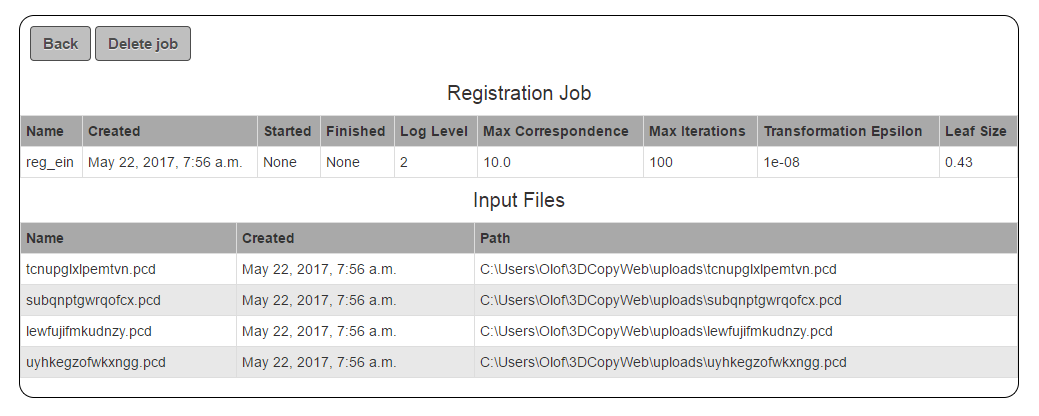
\includegraphics[width=160mm]{images/view_job.PNG}
		\caption{Information om ett job.}
		\label{fig:view_job}
	\end{figure}

	Förutom att se vilka parametrar som sattes på jobbet så kan man även se vilka filer som lades till. För att komma tillbaka till standardvyn så trycker man på \textit{Back}. Man kan även ta bort jobbet genom att trycka på \textit{Delete job}.
	
	\subsubsection{Start Job}
	
	\textit{Start Job} är den andra knappen som ett jobb har i listan. För att köra ett jobb så trycker man på \textit{Start Job}. Ett jobb kommer alltså inte att köras förrän någon har tryckt på \textit{Start Job}.
	
	\subsubsection{Delete Job}
	
	\textit{Delete Job} är den tredje och sista knappen som ett jobb har. Genom att trycka på \textit{Delete Job} så tar man bort jobbet ur listan. Jobbet tas även bort ur databasen och alla filer på serven som förknippas med jobbet tas också bort.
	
	\subsection{Att använda kommandoradsgränsnittet}
		För att använda programmet 3DCopy så kör man kommandot:
		
		\texttt{./3DCopy pcdfile1 pcdfile2 pcdfile3 ... outputfile}
		
		Där godtyckligt antal pcdfiler kan väljas. Dessa punktmoln kommer sedan att registreras och efter det kommer en mesh att genereras med \textit{outputfile} som det givna filnamnet. Ett exempel på hur man använder programmet från kommandoraden ser ut såhär:
		
		\texttt{./3DCopy pcd\_file\_1 pcd\_file\_2 result}
		
		Detta kommer alltså att generera en mesh med filnamn \textit{result} som sparas i ett .stl format. Denna fil kan sedan användas för att inspekteras i till exempel meshlab eller liknande program. Det går också att skriva ut objektet med en 3D-skrivare. Det som är värt att nämna är att programmet kan även ta in en mapp fylld med pcd-filer istället för enstaka pcd-filer som ska behandlas. Programmet söker då automatisk igenom mappen och plockar ut de filer som ska registreras, exempel på hur detta ser ut:
		
		\texttt{./3DCopy map\_with\_files result}
		
		Programmet 3DCopy innehåller ett antal underkommandon enligt formen
		
		\texttt{./3DCopy [kommando] pcdfile1 pcdfile2 pcdfile3 ... outputfile}
		
		Detta ger en möjlighet för användaren att välja vilken komponent som ska köras. Användaren kan enbart välja att köra meshningskomponenten eller registreringskomponenten. De kommandon som finns tillgängliga beskrivs nedan i tabell \ref{tab:flaggor_cli}.
		
		\begin{table}[h!]
			\centering
			\caption{Flaggor/kommandon för CLI.}
			\label{tab:flaggor_cli}
			
			\begin{tabular}{p{0.2\linewidth}p{0.6\linewidth}}
				Flagga & Förklaring \\
				\hline
				\texttt{-m} & Enbart mesha objektet utifrån ett givet komplett punktmoln. \\
				\hline
				\texttt{-r} & Enbart registrera punktmoln för att generera ett komplett punktmoln, hoppar över meshningen. \\
				\hline
				\texttt{-v} & Gör att programmet talar om mer nödvändig information om vad som händer till användaren. \\
				\hline
			\end{tabular}
		\end{table}	
		
		För att enbart registrera punktmoln kan således detta kommando användas:
		
		\texttt{./3DCopy -r pcdfile1 pcdfile2 pcdfile3 ... outputfile}
\newpage
   
    
\section{Installation}
\subsection{Installationsskript}
	För att installera systemen 3DCopy och filtret tillhandahålls ett installationsskript. Skriptet kan användas för att installera systemen på en dator som kör Ubuntu.
	
	För att installera installera 3DCopy måste koden först hämtas vilket kan göras med följande kommando:
	
	\texttt{git clone https://github.com/PUM-9/3DCopy.git \\
	cd 3DCopy}
	
	Kör sedan installationsskriptet:
	
	\texttt{./install.sh}
	
	För att installera filtret används samma metod:
	
	\texttt{git clone https://github.com/PUM-9/filter.git \\
	cd filter \\
	./install.sh}
	
	TreeD-Wrapper har inget installationsskript men för att använda det, kör
	
	\texttt{git clone https://github.com/PUM-9/treed\_wrapper.git}
	
	Själv skriptet som kör TreeD-Wrapper ligger sedan i \texttt{./treed\_wrapper/src/treed\_wrapper.py}. Det kan antingen köras direkt därifrån eller läggas i någon mapp som ligger i användarens sökväg (\texttt{PATH}) för att vara åtkomligt var som helst i systemet.
	
\subsection{Bygga själv}
	Om man använder ett annat system än Ubuntu är det inte säkert att installationsskriptet fungerar. Då kan man behöva bygga systemet själv.
	
	Till att börja med måste man installera alla beroenden. Se till att systemet har PCL, Boost och CMake installerat. Se även till att systemet har alla paket som behövs för att kompilera C++. Hämta sedan hem koden genom
	
	\texttt{git clone https://github.com/PUM-9/3DCopy.git}
	
	och ställ dig i mappen med
	
	\texttt{cd 3DCopy}
	
	Skapa sedan en mapp för alla byggfiler och ställ dig i den genom att köra
	
	\texttt{mkdir build \\
	cd build}
	
	Kör sedan CMake för att generera byggfiler för ditt system:
	
	\texttt{cmake ..}
	
	Till sist, bygg och installera 3DCopy genom att köra
	
	\texttt{make \\
	sudo make install}

	Motsvarande metod används för att bygga filtret men koden hämtas istället med kommandot
	
	\texttt{git clone https://github.com/PUM-9/filter.git}
\newpage

\end{document}

